\section{Análisis del problema}

    En este apartado explicaremos el funcionamiento del videojuego clásico Pac-Man, las bases y componentes del juego, el diseño de los niveles y el comportamiento de los fantasmas. También haremos una propuesta que cumpla con los objetivos específicos presentados en la primera sección, centrándonos principalmente en definir los apartados del juego en los que aplicaremos \acrshort{pcg}.

\subsection{Videojuego clásico escogido: Pac-Man}

    Hemos decidido escoger para su reimplementación aplicando técnicas de generación procedimental al videojuego Pac-Man \cite{officialSitePacman}, publicado en 1980 por la empresa Bandai Namco Entertainment Inc., conocido por todo el mundo y probablemente uno de los juegos más icónicos de todos los tiempos. Desde entonces se ha publicado multitud de contenido relacionado con esta franquicia, comenzando por decenas de nuevos videojuegos basados en el juego original, pasando por merchandising e incluso otro tipo de contenido como la guía \textit{Mastering Pac-Man} \cite{uston}, escrita por Ken Uston en 1981 en la que desvelaba todos los secretos del juego.\\
    
    Debido al hito en la historia de los videojuegos que supuso Pac-Man, a que las mecánicas y funcionamiento del juego pueden suponer un reto interesante a la hora de implementarlo, a que debido a que el juego original no utilizaba técnicas de generación procedimental y que el contenido del juego es apto para generarlo procedimentalmente (especialmente los laberintos), se ha decido escoger este juego. Para esta sección seguiremos el informe realizado por Jamey Pittman \cite{pittman2015} y la guía publicada por el usuario de Steam \textit{Night Druid} \cite{druid2016}. 
    
    \begin{figure}[H]
    \centering
        \begin{subfigure}[b]{0.49\textwidth}
        \centering
            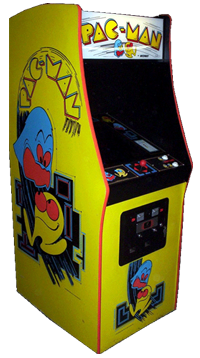
\includegraphics[width=3.3cm]{img/cabinet3.png}
            \caption{Máquina recreativa del videojuego original.}
        \end{subfigure}
        \hfill
        \begin{subfigure}[b]{0.49\textwidth}
        \centering
            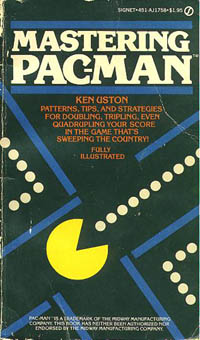
\includegraphics[width=3.3cm]{img/pbook.jpg}
            \caption{Guía escrita por Ken Uston.}
        \end{subfigure}
        \caption{Ejemplos de contenido relacionado con la franquicia de \textit{Pac-Man}. Imágenes obtenidas de \cite{pittman2015}.}
    \end{figure}

\subsubsection{Objetivo del juego}

El objetivo del juego es recorrer un laberinto comiéndonos todos los puntos situados a lo largo del mismo mientras escapamos de cuatro enemigos, los fantasmas. Si nos comemos todos los puntos, avanzamos de nivel, y si nos atrapan los fantasmas, perdemos una vida y se reiniciará la posición de Pac-Man y los fantasmas. Como ayuda contra los fantasmas, Pac-Man podrá utilizar un potenciador que le proporcionará invencibilidad y le permitirá derrotar a los fantasmas. Si derrotamos a un fantasma, volverá a su zona de inicio y reaparecerá para volver a perseguir a Pac-Man.

\subsubsection{Diseño de niveles}

El juego está compuesto por Pac-Man, el personaje amarillo; los 4 fantasmas, cada uno de un color (rojo, azul, rosa y naranja); laberinto (los pasillos y los muros), con una sección que llamaremos la ``casa'' de los fantasmas; 244 puntos y 4 potenciadores. Además, el laberinto contará con una conexión que unirá la parte derecha e izquierda del escenario, que llamaremos \textit{teletransportes}.

 \begin{figure}[H]
    \centering
        \begin{subfigure}[b]{0.4\textwidth}
        \centering
            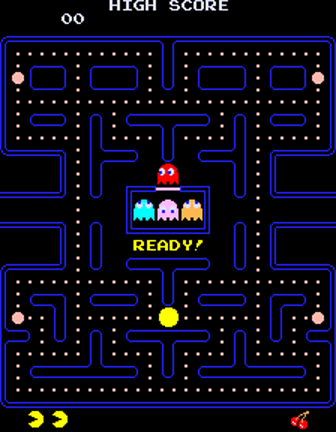
\includegraphics[width=5cm]{img/lvl1.png}
        \caption{Diseño de los niveles del 0 al 255.}
        \end{subfigure}
        \hspace{1cm}
        \begin{subfigure}[b]{0.4\textwidth}
        \centering
            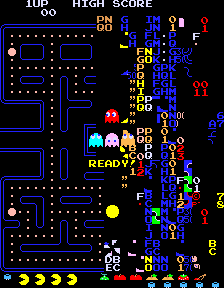
\includegraphics[width=5cm]{img/Level 256.png}
            \caption{Error del nivel 256.}
        \end{subfigure}
        \caption{Diseño de niveles del videojuego de \textit{Pac-Man}. Imágenes obtenidas de \cite{pittman2015}.}
        \label{fig:niveles}
    \end{figure}

En el juego original, a pesar de que existe una progresión de niveles, el escenario no cambia entre niveles, contando siempre con la misma disposición del laberinto (incluyendo las posiciones de los fantasmas, Pac-Man y los teletransportes) y distribución de los puntos y los potenciadores. Como curiosidad, cuando los jugadores alcanzaban el nivel 256, la capacidad de los registros de la CPU no era suficiente y ocasionaba que el juego generase lo que los jugadores bautizaron como ``pantalla de muerte'' o ``pantalla dividida''. Podemos ver un ejemplo en la figura \ref{fig:niveles}.

\subsubsection{Comportamiento de los fantasmas}

Aunque cada fantasma cuenta con un comportamiento propio, todos y cada uno de ellos comparten ciertas características. En primer lugar, los fantasmas van intercalando entre dos estados, perseguir y dispersarse, en ambos estados se dirigen hacia una casilla concreta del mapa. En el estado de perseguir esta casilla varía en función de cada fantasma y en el estado de dispersarse, cada fantasma cuenta con una zona por la que rondar.\\

Además, a la hora de decidir que ruta seguir, los fantasmas únicamente miran las casilla siguiente, tomando la decisión que le acerque más a su objetivo de un modo lineal, por lo que en ocasiones, dos o más decisiones supondrían la misma distancia lineal, siendo necesario establecer un orden de preferencia en las intersecciones de: arriba, izquierda, abajo y derecha. Esto ocasiona situaciones en las que aunque es evidente para un jugador que una de las dos rutas es más corta, el fantasma elija la menos eficiente, como ocurre en el ejemplo de la figura \ref{fig:decidir}.

\begin{figure}[H]
    \begin{center}
        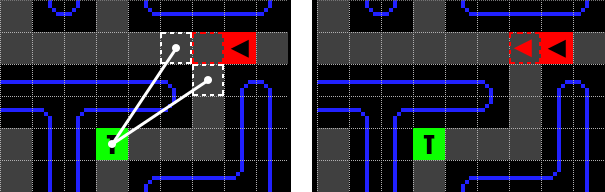
\includegraphics[scale=0.5,]{img/TieBreak.png}
        \caption{Resolución de conflicto de los fantasmas cuando la distancia es la misma. La casilla roja es el fantasma y su dirección y la verde su objetivo. Imagen obtenida de \cite{pittman2015}.}
        \label{fig:decidir}
    \end{center}
\end{figure}

En cuanto al comportamiento individual de cada fantasma entramos en detalle a continuación:

\begin{itemize}
    \item \textbf{Rojo:} es el fantasma que cuenta con un comportamiento más simple, ya que fija como casilla objetivo la posición actual de Pac-Man. Por ello se le considera el fantasma más agresivo de los cuatro. Podemos ver un ejemplo en la figura \ref{fig:red-pink}(a).
    \item \textbf{Rosa:} cuenta con otro comportamiento relativamente simple, ya que fija como casilla objetivo la casilla que se encuentre a cuatro unidades de distancia de la dirección actual de Pac-Man. Esto provoca que este fantasma se dirija generalmente hacia donde se esté moviendo el jugador. Podemos ver un ejemplo en la figura \ref{fig:red-pink}(b).
    \item \textbf{Azul:} utiliza la predicción que usa el fantasma rosa sumado a que traza un segmento cuyo origen es la posición del fantasma rojo, tiene por centro la casilla de la predicción y acaba en la casilla destino. Esto provoca que el fantasma nos encierre y se acerque más cuanto más cerca esté el rojo. Podemos ver un ejemplo en la figura \ref{fig:red-pink}(c).
    
     \begin{figure}[H]
    \centering
        \begin{subfigure}[b]{0.25\textwidth}
            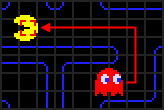
\includegraphics[scale=0.8]{img/red.png}
        \caption{Comportamiento del fantasma rojo.}
        \end{subfigure}
        \hspace{2cm}
        \begin{subfigure}[b]{0.25\textwidth}
            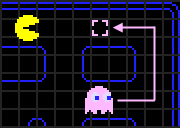
\includegraphics[scale=0.69]{img/pink.png}
            \caption{Comportamiento del fantasma rosa.}
        \end{subfigure}
        \vspace{0.5cm}
        \\
        \begin{subfigure}[b]{0.25\textwidth}
        \centering
            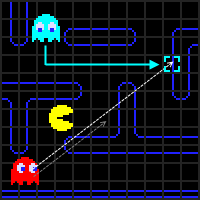
\includegraphics[scale=0.6]{img/blue.png}
            \caption{Comportamiento del fantasma azul.}
        \end{subfigure}
        \caption{Ejemplos de comportamiento de los fantasmas rojo, rosa y azul. Imágenes obtenidas de \cite{druid2016}.}
        \label{fig:red-pink}
    \end{figure}
    
    \item \textbf{Naranja:} quizás es el fantasma con el comportamiento más inofensivo para Pac-Man ya que aunque cuando se encuentra a más de 8 casillas de distancia, se comporta como el fantasma rojo y se dirige a la casilla actual de Pac-Man, cuando entra en ese radio, huye y se comporta similar a cuando se está dispersando.
\end{itemize}

\begin{figure}[H]
    \begin{center}
        \begin{subfigure}[b]{0.49\textwidth}
        \centering
            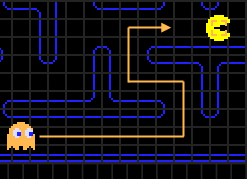
\includegraphics[scale=0.6]{img/orange1.png}
            \caption{Comportamiento de persecución.}
        \end{subfigure}
        \hfill
        \begin{subfigure}[b]{0.49\textwidth}
        \centering
            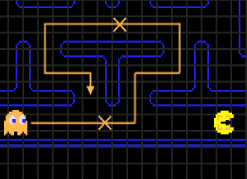
\includegraphics[scale=0.6]{img/orange2.png}
            \caption{Comportamiento de huida.}
        \end{subfigure}
        \caption{Ejemplo de comportamiento del fantasma naranja. Imágenes obtenidas de \cite{druid2016}.}
        \label{fig:blue}
    \end{center}
\end{figure}

% ---------------------------------------------------------------------------- %
\newpage
\subsection{Propuesta}

    El grueso de este proyecto y el objetivo principal del mismo es la aplicación de generación procedimental de contenido \acrshort{pcg} al videojuego clásico Pac-Man. Para ello, se propone aplicar técnicas de \acrshort{pcg} al mapeado, en particular al laberinto, las texturas y la inteligencia artificial del juego.

\subsubsection{Generación de laberintos}

    En particular, implementaremos un algoritmo que genere laberintos para dicho juego. Cuando hablamos de laberintos no solo hablamos de los caminos y muros, sino del nivel al completo del juego, incluyendo otros elementos como por ejemplo los puntos que debe comerse Pac-Man.\\
    
    Siguiendo la clasificación de contenido generado procedimentalmente que hemos establecido en la sección anterior, nuestro problema cae directamente en las categorías de \textit{Game Design}, debido a que los laberintos generados compondrán un nivel del juego, y, principalmente de \textit{Game Systems}, en la subcategoría \textit{Redes de carreteras}. Esto se debe a que nuestro problema no es más que la generación de una serie de caminos en el que se mantiene un equilibrio entre la aleatoriedad de los mismos y una estructura lógica y restricciones en cuanto a la disposición de los elementos que componen el laberinto.\\
    
    Para ello partiremos del método desarrollado en la propuesta e implementación de Shaun LeBron \cite{lebron2012}, creando un modelo y algoritmo propio para la generación procedimental de laberintos del juego Pac-Man.

\subsubsection{Generación de texturas}

    Con el fin de explorar técnicas de generación procedimental de contenido a diversos niveles dentro de la clasificación realizada, se propone explorar la Teselación de Voronoi como método de generación de texturas que aplicaremos a los muros de nuestro escenario.\\
    
    Siguiendo la clasificación de contenido generado procedimentalmente que hemos establecido en la sección anterior, nuestro problema cae directamente en la categoría de \textit{Game Bits}, debido a que las texturas forman parte de las unidades más básicas de contenido que componen un juego.

\subsubsection{Comportamiento de la inteligencia artificial}

    Teniendo en cuenta que el desarrollo de una inteligencia artificial similar a la del juego Pac-Man no es el objetivo de este proyecto, se propone desarrollar una versión simplificada de la misma. Concretamente, se implementará una máquina de estados que defina el comportamiento que deben tomar los fantasmas en cada momento y en lo que a algoritmos de búsqueda de caminos se refiere, utilizaremos el algoritmo de búsqueda A estrella (de ahora en adelante \acrshort{astar}, con su traducción en inglés, \acrlong{astar}).\\
    
    En cuanto a \acrshort{pcg}, alteraremos el comportamiento de los fantasmas mediante parámetros que generaremos procedimentalmente teniendo en cuenta diversos factores como por ejemplo, el nivel actual o la habilidad del jugador. Algunos ejemplos de parámetros que modificarían el comportamiento de los fantasmas sería la agresividad o la persistencia a la hora de perseguir al jugador.